\selectlanguage{italian}%

\section{Soluzione}


\subsection{Schematici}

La seguente Boundary Scan Chain � realizzata a partire da quattro
flip flop edge triggered che in ingresso prendono l'uscita di un multiplexer
che, pilotato da un segnale di \textit{scan\_en}, decide di selezionare
o un ingresso utente \textit{din} oppure l'uscita del flip flop precedente.
Quindi quando scan\_en � basso il sistema funziona in modalit� registro,
conservando il dato din, altrimenti funziona da shift-register, shiftando
i valori in ingresso al segnale \textit{scan\_in}, fino a quello di
scan\_out dopo un numero di colpi di clock pari al numero di registri.

\begin{figure}[H]
	\centering
	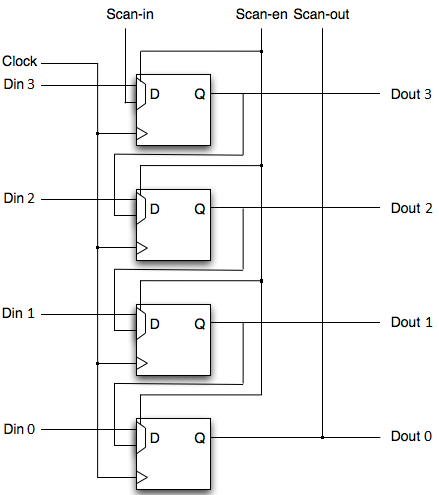
\includegraphics[scale=0.8]{esercizio06/images/scan_chain.png}
	\caption{Boundary Scan Chain}
	\label{fig:scan_chain}
\end{figure}

\subsection{Codice}

Progetto ISE: \href{run:progetti/Boundary_Scan_Chain/Boundary_Scan_Chain.xise}{Boundary Scan Chain ISE}


\subsubsection{Boundary\_Scan\_Chain}

Questo componente � stato realizzato con un approccio Structural,
componendo opportunamente dei flip-flop d edge triggered e dei mux
2-1. In particolare � stato utilizzato un secondo segnale di abilitazione
\textit{en} oltre a \textit{scan\_en}: il primo, quando � basso, attiva
la modalit� registro e quindi uno dei due ingressi del mux \textit{dinapp}
viene caricato con l'ingresso utente \textit{din} e mostrato poi all'uscita
\textit{dout} dei flip flop, mentre quando � alto abilita la modalit�
di shift register che, nel caso in cui scan\_en � basso viene utilizzata
per shiftare il valore din, che se non usassi questa doppia abilitazione
perderei( per ottenere lo stesso risultato dovrei caricare la scan
chain serialmente, questa piccola modifica ci servir� successivamente),
e nel caso in cui scan\_en � alto viene utilizzata per shiftare un
valore messo in ingresso al segnale di \textit{scan\_in}, che sar�
visibile poi all'uscita scan\_out dopo un certo numero di colpi di
clock. Infine per concatenare l' uscita di ogni flip flop con l'ingresso
del mux successivo, � stato utilizzato il segnale \textit{q}. \\
\lstinputlisting [language=VHDL,caption={Definizione della Boundary Scan Chain}] {progetti/Boundary_Scan_Chain/boundary_scan_chain.vhd}\selectlanguage{italian}%

